\documentclass[tikz,border=8pt]{standalone}
% Shared look for every TikZ diagram. Load with \input{../../tools/tikz-style.tex}
\usepackage[T1]{fontenc}
\usepackage{lmodern}
\renewcommand{\sfdefault}{lmr}  % diagrams use the same serif as the text
\usetikzlibrary{arrows.meta, positioning, shapes.geometric, calc, fit, backgrounds}
\definecolor{cblue}{HTML}{4C78A8}
\definecolor{corange}{HTML}{F58518}
\definecolor{cgreen}{HTML}{54A24B}
\definecolor{cred}{HTML}{E45756}
\definecolor{cpurple}{HTML}{B279A2}
\definecolor{cgrey}{HTML}{6B6B6B}
\tikzset{
  every picture/.style={font=\sffamily, line width=1.2pt},
  box/.style={draw=#1, fill=#1!12, rounded corners=4pt, align=center, inner sep=7pt, minimum height=1.1cm},
  box/.default=cgrey,
  arrow/.style={-{Stealth[length=3mm]}, draw=cgrey, line width=1.4pt},
  title/.style={font=\sffamily\bfseries\Large},
  note/.style={font=\sffamily\small, text=cgrey, align=center},
}
\AtBeginDocument{\hyphenpenalty=10000 \exhyphenpenalty=10000}

% State transition probability for the command "move 2": from cell 1 the robot ends in cell 2, 3 or 4 with
% probability 0.1, 0.8, 0.1. Every cell has the same three arrows, shifted.
\definecolor{cbrown}{HTML}{9C755F}
\begin{document}
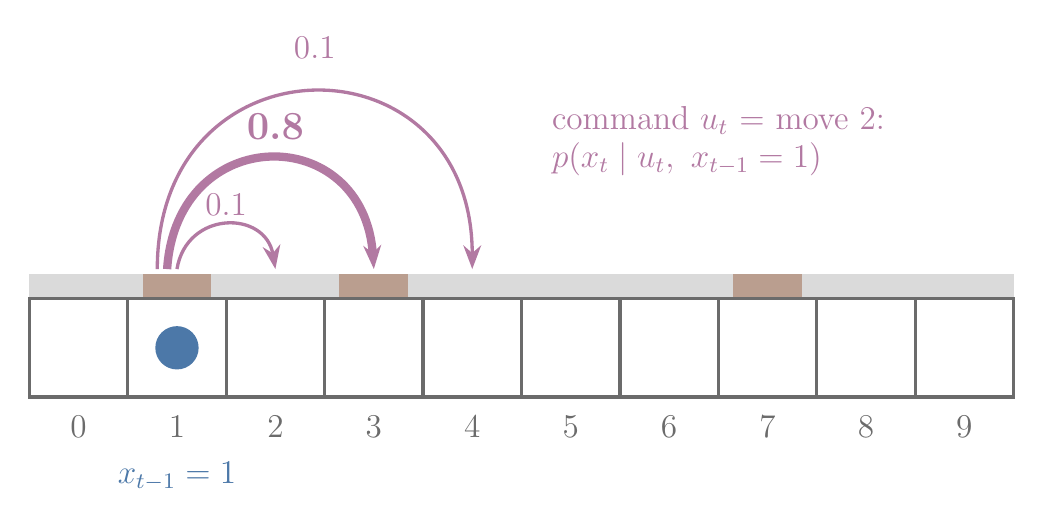
\begin{tikzpicture}[x=1.25cm, y=1.25cm, every node/.append style={font=\large}]
  \fill[cgrey!25] (0,1) rectangle (10,1.25);
  \foreach \d in {1,3,7} {\fill[cbrown!70] (\d+0.15,1) rectangle (\d+0.85,1.25);}
  \foreach \i in {0,...,9} {
    \draw[cgrey] (\i,0) rectangle (\i+1,1);
    \node[cgrey] at (\i+0.5,-0.3) {\i};
  }
  \fill[cblue] (1.5,0.5) circle (0.22);
  \node[cblue, anchor=north] at (1.5,-0.55) {$x_{t-1} = 1$};
  \draw[arrow, cpurple, line width=1.2pt] (1.5,1.3) .. controls (1.6,1.9) and (2.4,1.9) .. (2.5,1.3);
  \node[cpurple] at (2.0,1.95) {0.1};
  \draw[arrow, cpurple, line width=3pt] (1.4,1.3) .. controls (1.5,2.8) and (3.4,2.8) .. (3.5,1.3);
  \node[cpurple, font=\Large\bfseries] at (2.5,2.75) {0.8};
  \draw[arrow, cpurple, line width=1.2pt] (1.3,1.3) .. controls (1.3,3.7) and (4.5,3.7) .. (4.5,1.3);
  \node[cpurple] at (2.9,3.55) {0.1};
  \node[cpurple, anchor=west, align=left] at (5.2,2.6) {command $u_t$ = move 2:\\$p(x_t \mid u_t,\ x_{t-1} = 1)$};
\end{tikzpicture}
\end{document}
